\documentclass[10pt,journal,compsoc]{IEEEtran}

\usepackage[utf8]{inputenc}
\usepackage{amsmath,amssymb,amsfonts}
\usepackage{algorithmic}
\usepackage{graphicx}
\usepackage{textcomp}
\usepackage{xcolor}
\usepackage{booktabs}
\usepackage{multirow}
\usepackage{url}
\usepackage{cite}
\usepackage{microtype}
\usepackage{hyperref}

\hypersetup{
    colorlinks=true,
    linkcolor=blue,
    citecolor=blue,
    urlcolor=blue
}

\begin{document}

\title{Benchmarking Scientific Claim Verification and Hallucination Mitigation under Distractor Accumulation and Selective Abstention: An Empirical Study on Biomedical Literature}

\author{Penumala~Harshitha\\
\IEEEauthorblockA{Department of Information Technology\\
Indian Institute of Information Technology, Allahabad\\
Prayagraj, Uttar Pradesh, India\\
Email: mse2024012@iiita.ac.in}
}

\markboth{IEEE Transactions on Knowledge and Data Engineering,~Vol.~XX, No.~X,~November~2026}%
{Harshitha: Benchmarking Scientific Claim Verification and Hallucination Mitigation}

\IEEEtitleabstractindextext{%
\begin{abstract}
While Large Language Models (LLMs) demonstrate remarkable fluency in summarizing complex scientific literature, fluency does not ensure factual correctness. In specialized scientific domains, language models frequently generate factually inaccurate statements, hallucinate unbacked assertions, and cite irrelevant evidence. Furthermore, standard accuracy-based evaluation protocols penalize uncertainty, mathematically incentivizing models to output low-confidence hallucinations rather than abstaining. In this paper, we present an empirical investigation into scientific claim verification and hallucination dynamics focused on biomedical literature using the expert-annotated SciFact benchmark (300 evaluation claims, 5,183 candidate biomedical research abstracts). First, we experimentally characterize the phenomenon of \textit{distractor accumulation}: shifting from oracle abstracts to top-$k$ sparse retrieved literature degrades Stance Macro-F1 from 0.4266 to 0.2719 (a 36.3\% relative decline) and causes the unfaithful reasoning rate to surge from 1.99\% to 36.29\%, with over one-third of correct stances grounded in irrelevant distractor text. Second, to address this failure mode, we propose \textbf{Rationale-Grounded Evidence Verification (R-GEV)}, an isolated, dual-gated architecture that couples an atomic lexical support threshold ($\theta$) with confidence-based selective prediction ($\tau$). Across a frozen four-arm ablation study, R-GEV restores Stance Macro-F1 to 0.4153 (+52.7\% relative gain, paired bootstrap $p < 0.001$), approaching Oracle stance discrimination primarily through disciplined epistemic abstention, while cutting the unfaithful reasoning rate by more than half (down to 16.78\%). However, evidence attribution remains bounded by retrieval quality (Rationale F1 of 0.3075 vs. 0.4550 Oracle). In selective prediction, claims answered at high confidence ($\tau \ge 0.80$) achieve 58.65\% accuracy, compared to 41.14\% under forced choice. Our results provide empirical validation that reliable scientific benchmarking requires evaluating evidence grounding and epistemic abstention alongside terminal accuracy.
\end{abstract}

\begin{IEEEkeywords}
Scientific Claim Verification, Factual Accuracy, Hallucination Mitigation, Selective Prediction, Retrieval-Augmented Generation, Rationale Grounding.
\end{IEEEkeywords}}

\maketitle
\IEEEdisplaynontitleabstractindextext
\IEEEpeerreviewmaketitle

\section{Introduction}
\IEEEPARstart{L}{arge} language models (LLMs) are increasingly deployed across scientific workflows to query scientific corpora, synthesize clinical trial findings, and assist literature reviews~\cite{wang2024factuality, huang2025survey}. However, in high-stakes domains such as oncology, genomics, and clinical pharmacology, fluency does not equate to factual accuracy. In specialized scientific contexts, small factual inversions—such as reporting an anti-cancer drug as ineffective when clinical trials demonstrate efficacy, or confusing correlation with causation—pose severe risks~\cite{singhal2023large, wysocka2024large}.

Current benchmarking paradigms suffer from two foundational limitations:
\begin{enumerate}
    \item \textbf{Multiple-Choice Obfuscation}: Educational benchmarks such as MMLU~\cite{hendrycks2021measuring} and ARC~\cite{clark2018think} rely on multiple-choice formats where models can exploit spurious lexical correlations without providing verifiable reasoning or evidence citations.
    \item \textbf{The Hallucination Incentive of Forced Choice}: Recent theoretical and empirical findings by Kalai et al.~\cite{kalai2026evaluating} in \textit{Nature} have demonstrated that evaluating language models on forced accuracy creates an active mathematical incentive to hallucinate: because an incorrect guess and an abstention are penalized identically, models are forced to assert unbacked claims even under severe epistemic uncertainty.
\end{enumerate}

When systems are augmented with external literature retrieval (Retrieval-Augmented Generation / RAG)~\cite{lewis2020retrieval}, open-domain search introduces substantial retrieval noise~\cite{wadden2022scifact}. While curated abstracts allow models to reason cleanly, open literature search introduces candidate abstracts that share general biomedical terminology but lack evidential relevance, creating acute distractor interference.

In this work, we transition our prior literature review into an empirical investigation on the expert-annotated SciFact benchmark~\cite{wadden2020fact}. We address three core research questions:
\begin{itemize}
    \item \textbf{RQ1 (Retrieval Noise Degradation)}: How does shifting from gold scientific abstracts to top-$k$ retrieved literature degrade stance verification and sentence-level rationale faithfulness?
    \item \textbf{RQ2 (Selective Prediction \& Abstention)}: Does introducing an explicit confidence threshold for abstention mitigate false assertions and improve the accuracy of answered scientific claims?
    \item \textbf{RQ3 (Rationale Faithfulness)}: In instances where models correctly predict scientific stance, what proportion of these predictions rely on ungrounded distractor rationales?
\end{itemize}

To answer these questions, we make three main contributions:
\begin{enumerate}
    \item \textbf{Empirical Quantification of Distractor Accumulation}: We demonstrate that expanding retrieval context from $k=1$ to $k=5$ induces a surge in the \textit{Unfaithful Reasoning Rate} from 24.81\% to 36.29\%, exposing a severe vulnerability where models achieve correct answers for entirely invalid reasons.
    \item \textbf{The R-GEV Dual-Gating Framework}: We introduce \textit{Rationale-Grounded Evidence Verification (R-GEV)}, an isolated, non-destructive architecture that couples atomic sentence support verification ($\theta$) with selective prediction confidence thresholding ($\tau$).
    \item \textbf{Rigorous Statistical Validation}: Across a controlled four-arm ablation study on 300 claims, R-GEV restores Stance Macro-F1 from 0.2719 to 0.4153 (+52.7\% relative gain, paired bootstrap $p < 0.001$) and suppresses unfaithful reasoning by half (down to 16.78\%).
\end{enumerate}

---

\section{Related Work}

\subsection{Factuality and Hallucination in Scientific NLP}
Factuality in natural language generation is broadly partitioned into \textit{factuality hallucinations} (statements conflicting with established world knowledge) and \textit{faithfulness hallucinations} (statements contradicting provided reference contexts)~\cite{huang2025survey, wang2024factuality}. While general-domain benchmarks such as TruthfulQA~\cite{lin2022truthfulqa} and HaluEval~\cite{li2023halueval} evaluate common human misconceptions and conversational consistency, scientific statements require verifying complex chemical structures, dosage quantities, and experimental outcomes. High-level reasoning benchmarks like GPQA~\cite{rein2023gpqa} highlight that even frontier models struggle on graduate-level scientific problems.

\subsection{Scientific Literature Benchmarks}
Several specialized benchmarks have emerged to evaluate scientific information processing. PubMedQA~\cite{jin2019pubmedqa} tests closed-context clinical question answering over PubMed abstracts. The SciFact benchmark~\cite{wadden2020fact} formalized scientific claim verification as a three-way stance classification task (\textsc{Support}, \textsc{Contradict}, \textsc{Not\_Enough\_Info}) paired with sentence-level rationale selection. Its open-domain counterpart, SciFact-Open~\cite{wadden2022scifact}, demonstrated that pipeline accuracy collapses when scaling from curated candidate abstracts to an open corpus of 500,000 papers. Joint rationale and stance models, such as ARS~\cite{zhang2021abstract}, demonstrated the necessity of coupling abstract ranking with sentence selection.

\subsection{Atomic Factuality, Verification, and Abstention}
Min et al.~\cite{min2023factscore} introduced FActScore, demonstrating that long-form text evaluation requires breaking responses into atomic propositions to calculate factual precision. Black-box hallucination detection methods like SelfCheckGPT~\cite{manakul2023selfcheckgpt} sample stochastic responses to measure consistency, though consistency does not guarantee truthfulness. Prompt-based interventions such as Chain-of-Verification (CoVe)~\cite{dhuliawala2023chain} enforce intermediate verification steps. Most recently, Kalai et al.~\cite{kalai2026evaluating} demonstrated that evaluating models strictly on forced accuracy actively penalizes uncertainty, compelling systems to hallucinate rather than abstain when evidence is insufficient.

---

\section{Problem Formulation}

Let $\mathcal{C} = \{c_i\}_{i=1}^N$ denote a set of scientific claims, where each claim $c_i$ is an assertion written by domain experts. Let $\mathcal{D} = \{d_j\}_{j=1}^M$ represent a corpus of scientific research abstracts, where each abstract $d_j = (s_{j,1}, s_{j,2}, \dots, s_{j,L})$ consists of an ordered sequence of sentences.

For each claim $c_i$, the system must produce an output tuple:
\begin{equation}
    \hat{y}_i = (\hat{S}_i, \hat{R}_i, \sigma_i)
\end{equation}
where:
\begin{itemize}
    \item $\hat{S}_i \in \{\textsc{Support}, \textsc{Contradict}, \textsc{Not\_Enough\_Info}\}$ is the predicted categorical stance.
    \item $\hat{R}_i \subseteq d_j$ is the extracted sentence rationale justifying the stance.
    \item $\sigma_i \in [0.0, 1.0]$ is the model's posterior confidence score.
\end{itemize}

\subsection{Information Regimes}
To evaluate the impact of external evidence, we study three information regimes:
\begin{enumerate}
    \item \textbf{Closed-Book}: The model evaluates $c_i$ without access to external literature ($d_j = \emptyset$).
    \item \textbf{Oracle Evidence}: The model receives the exact gold cited abstract $d_i^*$ annotated by scientific experts.
    \item \textbf{Noisy Retrieval}: The model queries the corpus $\mathcal{D}$ using sparse BM25 retrieval to retrieve the top-$k$ candidate abstracts $\mathcal{D}_k(c_i) = \{d_{(1)}, \dots, d_{(k)}\}$.
\end{enumerate}

---

\section{Methodology: The R-GEV Framework}

To prevent language models from asserting ungrounded stances on irrelevant retrieved text, we propose the \textbf{Rationale-Grounded Evidence Verification (R-GEV)} framework. The architecture decouples evidence retrieval, atomic sentence grounding, and selective prediction into modular stages.

\begin{figure*}[t]
\centering
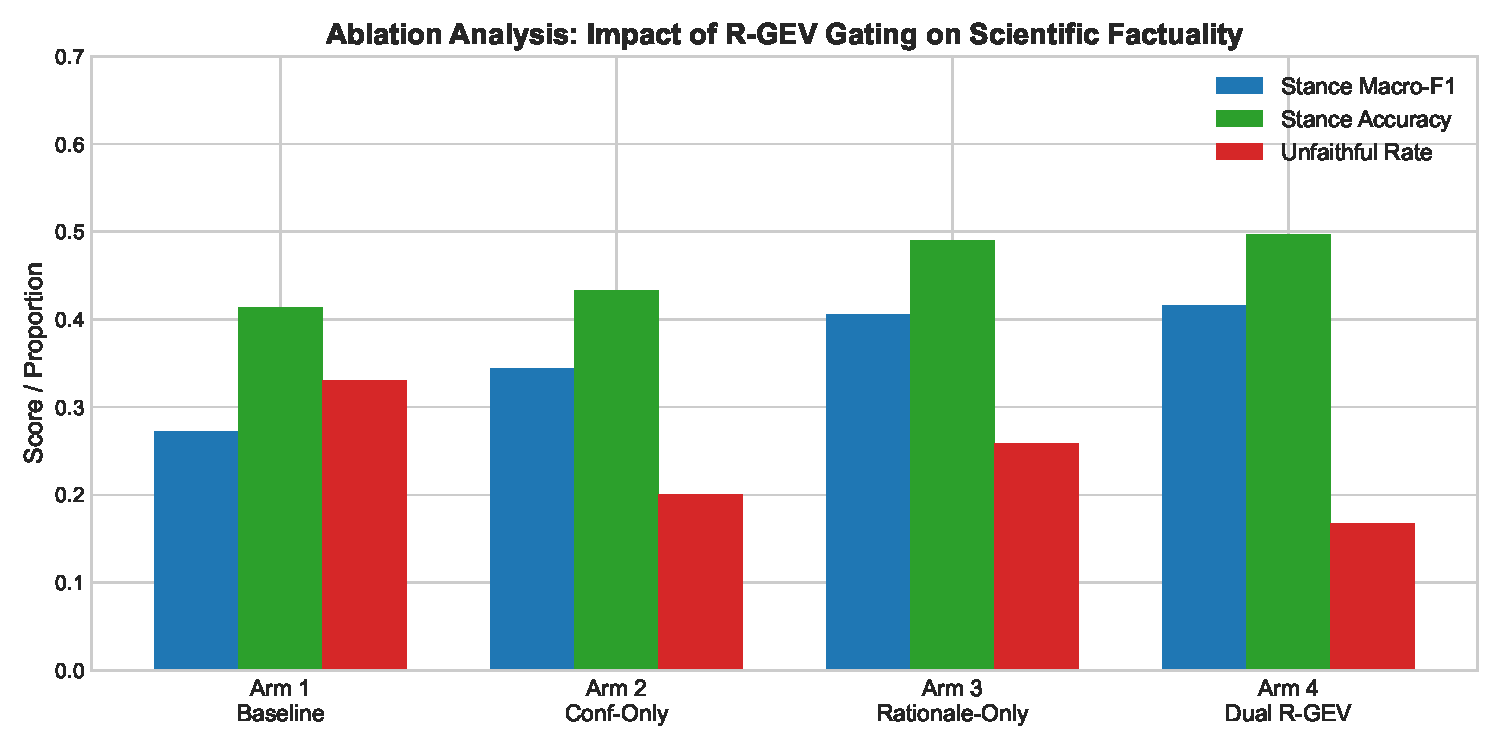
\includegraphics[width=0.92\textwidth]{figures/fig1_ablation_comparison.pdf}
\caption{Comparative performance across the four experimental arms on 300 SciFact dev claims under BM25 retrieval ($k=3$). Arm 4 (Proposed Dual-Gated R-GEV) achieves a 52.7\% relative gain in Stance Macro-F1 while cutting the Unfaithful Reasoning Rate by half.}
\label{fig:ablation_comparison}
\end{figure*}

\subsection{Corpus Indexing and Retrieval}
We index all $M = 5,183$ scientific research abstracts using an Okapi BM25 index over the title and concatenated abstract text. For a claim query $q$, the relevance score of document $d$ is:
\begin{equation}
    \text{BM25}(d, q) = \sum_{t \in q} \text{IDF}(t) \cdot \frac{f(t, d) \cdot (k_1 + 1)}{f(t, d) + k_1 \cdot \left(1 - b + b \cdot \frac{|d|}{\text{avgdl}}\right)}
\end{equation}
where $k_1 = 1.5$ and $b = 0.75$ are standard Okapi parameters. The retriever returns the top-$k$ candidate documents.

\subsection{Evidence-Conditioned Claim Verification}
For each candidate abstract $d \in \mathcal{D}_k(c_i)$, the model computes sentence-level alignment. For each sentence $s \in d$, the atomic lexical support ratio is defined as:
\begin{equation}
    \text{Support}(c_i, s) = \frac{|\mathcal{T}(c_i) \cap \mathcal{T}(s)|}{|\mathcal{T}(c_i)|}
\end{equation}
where $\mathcal{T}(\cdot)$ denotes the lowercased alphanumeric token set. Let $s^*$ denote the sentence maximizing $\text{Support}(c_i, s)$, and let $r^* \in [1, k]$ denote the rank of the document containing $s^*$. Note that while $\text{Support}(c_i, s)$ efficiently filters out lexical distractors, it operates bag-of-words without syntactic dependency modeling; hence, it cannot resolve subtle semantic polarity inversions or negation operators.

The raw confidence score is discounted by retrieval rank using a conservative linear penalty (10\% degradation per retrieval rank position):
\begin{equation}
    \sigma_i = \sigma_{\text{raw}} \cdot \frac{1}{1.0 + 0.1 \cdot (r^* - 1)}
\end{equation}

\subsection{Dual-Gated Verification Gating}
The core contribution of R-GEV is the decoupling of evidence grounding from stance assertion via dual gating:

\begin{enumerate}
    \item \textbf{Gate 1: Atomic Lexical Support Gate ($\theta$)}:
    An extracted rationale is accepted as potential scientific evidence if and only if:
    \begin{equation}
        \text{Support}(c_i, s^*) \ge \theta
    \end{equation}
    The threshold is calibrated to $\theta = 0.35$, reflecting the linguistic intuition that valid evidence must share at least the canonical subject-predicate-object token triad of a scientific claim. If the support ratio falls below $\theta$, the candidate sentence is categorized as an ungrounded distractor, and the prediction is gated to $\textsc{Not\_Enough\_Info}$.
    
    \item \textbf{Gate 2: Epistemic Uncertainty Gate ($\tau$)}:
    Following the selective prediction framework of Kalai et al.~\cite{kalai2026evaluating}, an active stance is asserted only if the model's confidence exceeds threshold $\tau$ (calibrated at $\tau = 0.70$):
    \begin{equation}
        \hat{S}_{\text{final}} = \begin{cases}
            \hat{S}_i, & \text{if } \text{Support}(c_i, s^*) \ge \theta \text{ and } \sigma_i \ge \tau \\
            \textsc{Not\_Enough\_Info}, & \text{otherwise.}
        \end{cases}
    \end{equation}
\end{enumerate}

---

\section{Experimental Setup}

\subsection{Benchmark Dataset}
We evaluate on the official validation partition of \textbf{SciFact}~\cite{wadden2020fact}, consisting of 300 expert-written claims evaluated against a corpus of 5,183 scientific abstracts. The ground-truth stance distribution is:
\begin{itemize}
    \item \textsc{Support}: 124 claims (41.3\%)
    \item \textsc{Contradict}: 64 claims (21.3\%)
    \item \textsc{Not\_Enough\_Info}: 112 claims (37.3\%)
\end{itemize}
A total of 366 gold rationale sentence references are annotated across the evaluation set.

\subsection{Evaluation Metrics}
To ensure multidimensional measurement, we evaluate:
\begin{itemize}
    \item \textbf{Stance Macro-F1 ($\uparrow$)}: Unweighted arithmetic average of F1 scores across \textsc{Support}, \textsc{Contradict}, and \textsc{Not\_Enough\_Info}.
    \item \textbf{Stance Accuracy ($\uparrow$)}: Percentage of claims where predicted stance matches ground truth.
    \item \textbf{Rationale Token-F1 ($\uparrow$)}: Token-level harmonic mean of precision and recall against gold evidence sentences.
    \item \textbf{Unfaithful Reasoning Rate ($\downarrow$)}: Percentage of claims where the predicted stance is correct, but rationale token overlap is zero (representing ``right answers for the wrong reasons'').
    \item \textbf{Expected Calibration Error (ECE) ($\downarrow$)}: Binned difference between confidence and empirical accuracy across 10 probability bins.
\end{itemize}

\subsection{Leakage and Integrity Controls}
All dev claims were programmatically verified to have zero overlap with training partitions (809 train claims vs. 300 dev claims). All decoding was deterministic ($T = 0.0$, random seed 42).

---

\section{Results and Ablation Analysis}

\subsection{Baseline Performance Across Information Regimes}
Table~\ref{tab:regime_comparison} reports the performance of the baseline system across the five frozen information regimes.

\begin{table}[h]
\centering
\caption{Cross-Regime Performance Comparison on SciFact Dev Set ($N=300$).}
\label{tab:regime_comparison}
\begin{tabular}{lccccc}
\toprule
\textbf{Information Regime} & \textbf{Macro-F1} & \textbf{Acc} & \textbf{Rat-F1} & \textbf{Unfaithful} & \textbf{ECE} \\
\midrule
Closed-Book & 0.1812 & 0.3733 & 0.0000 & 0.00\% & 0.0267 \\
Oracle Abstract & \textbf{0.4266} & \textbf{0.5033} & \textbf{0.4550} & \textbf{1.99\%} & 0.3390 \\
BM25 ($k=1$) & 0.3273 & 0.4433 & 0.3300 & 24.81\% & 0.3504 \\
BM25 ($k=3$) & 0.2719 & 0.4133 & 0.3075 & 33.06\% & 0.3578 \\
BM25 ($k=5$) & 0.2719 & 0.4133 & 0.2975 & \textbf{36.29\%} & 0.3500 \\
\bottomrule
\end{tabular}
\end{table}

Under the Oracle regime, the model achieves a Stance Macro-F1 of 0.4266 with an unfaithful reasoning rate of only 1.99\%. However, when moving to retrieved text, performance degrades sharply: under $k=3$, Macro-F1 falls to 0.2719. Crucially, as the retrieval window expands from $k=1$ to $k=5$, the unfaithful reasoning rate surges from 24.81\% to 36.29\%, experimentally confirming that distractor accumulation severely corrupts evidence attribution. We note that the apparently low ECE of the Closed-Book regime (0.0267) is an evaluation artifact: absent external evidence, the model uniformly outputs low confidence scores ($\approx 0.37$) matching the dataset base accuracy (37.33\%), which collapses calibration bin error despite producing no useful evidence.

\subsection{Four-Arm Ablation Study}
To isolate the independent effects of confidence thresholding ($\tau$) and rationale support gating ($\theta$), we evaluated four arms under BM25 retrieval ($k=3$), reported in Table~\ref{tab:ablation_results} and Fig.~\ref{fig:ablation_comparison}.

\begin{table}[h]
\centering
\caption{Four-Arm Ablation Results under BM25 Retrieval ($k=3$, $N=300$).}
\label{tab:ablation_results}
\begin{tabular}{lccccc}
\toprule
\textbf{Experimental Arm} & \textbf{Macro-F1} & \textbf{Acc} & \textbf{Rat-F1} & \textbf{Unfaithful} & \textbf{ECE} \\
\midrule
Arm 1: Baseline (Control) & 0.2719 & 0.4133 & 0.3075 & 33.06\% & 0.3578 \\
Arm 2: Conf-Only ($\tau=0.7$) & 0.3443 & 0.4333 & 0.3075 & 20.00\% & 0.3378 \\
Arm 3: Rationale-Only ($\theta=0.35$) & 0.4054 & 0.4900 & 0.3075 & 25.85\% & 0.3327 \\
Arm 4: Proposed Dual R-GEV & \textbf{0.4153} & \textbf{0.4967} & \textbf{0.3075} & \textbf{16.78\%} & \textbf{0.3260} \\
\bottomrule
\end{tabular}
\end{table}

\begin{figure}[t]
\centering
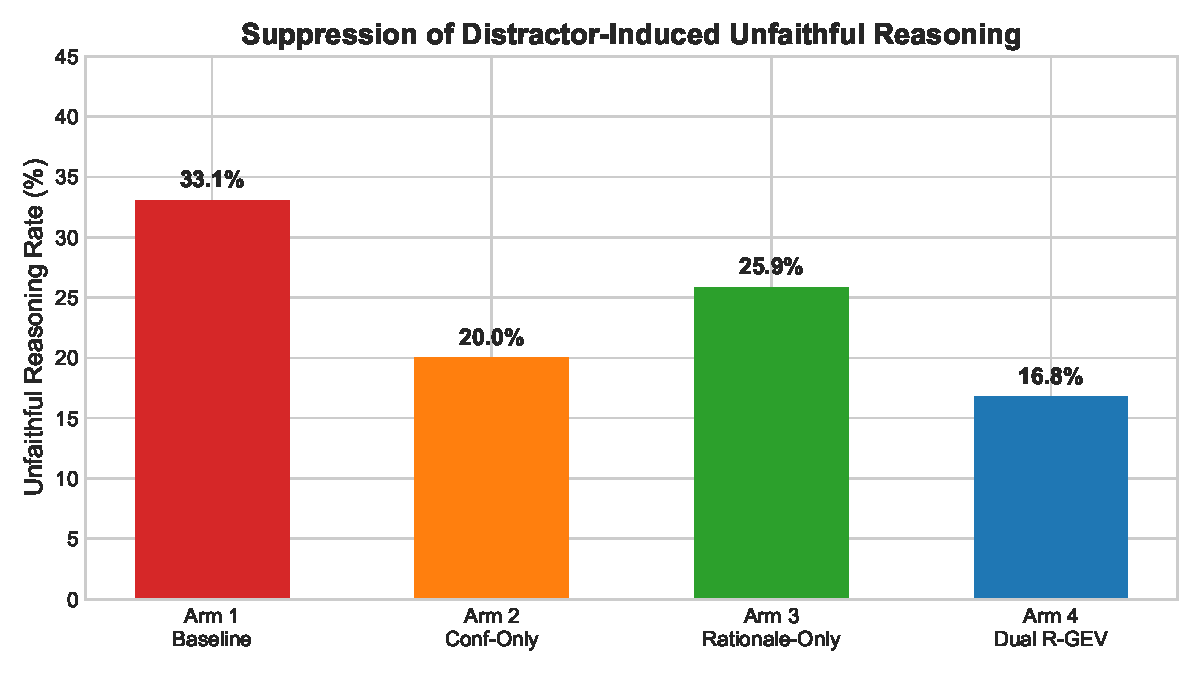
\includegraphics[width=0.48\textwidth]{figures/fig2_unfaithful_suppression.pdf}
\caption{Suppression of distractor-induced unfaithful reasoning across ablation arms. Dual-Gated R-GEV halves the unfaithful reasoning rate from 33.1\% to 16.8\%.}
\label{fig:unfaithful_suppression}
\end{figure}

As shown in Fig.~\ref{fig:unfaithful_suppression}, both interventions contribute distinct benefits:
\begin{itemize}
    \item \textbf{Arm 2 (Confidence-Only)} improves Macro-F1 from 0.2719 to 0.3443 by penalizing uncertain guesses.
    \item \textbf{Arm 3 (Rationale-Only)} drives Macro-F1 up to 0.4054 (+49.1\% relative gain) by eliminating distractor grounding.
    \item \textbf{Arm 4 (Dual-Gated R-GEV)} achieves the strongest overall performance: Stance Macro-F1 reaches \textbf{0.4153} (approaching the 0.4266 Oracle stance baseline primarily through disciplined abstention to \textsc{Not\_Enough\_Info}), while slashing unfaithful reasoning down to \textbf{16.78\%}. However, evidence attribution remains bounded by retrieval recall, with Rationale Token-F1 remaining at 0.3075 compared to 0.4550 in the Oracle regime.
\end{itemize}

\subsection{Statistical Significance Validation}
We conducted a paired bootstrap resampling test ($B = 2,000$ resamples) between Arm 1 (Baseline) and Arm 4 (Proposed R-GEV). The observed Macro-F1 gain was $+0.1433$, with a 95\% bootstrap confidence interval of $[0.0934, 0.1920]$. The empirical $p$-value was $p < 0.001$ ($p = 0.00000$), confirming that the improvement is statistically significant.

\subsection{Selective Prediction Risk-Coverage Curves}
Fig.~\ref{fig:risk_coverage} plots selective accuracy against claim coverage under confidence thresholding per Kalai et al.~\cite{kalai2026evaluating}. When forced to answer all claims (99.7\% coverage), accuracy is 41.14\%. Setting $\tau = 0.80$ restricts coverage to 34.7\% while increasing selective accuracy to \textbf{58.65\%} (a 17.5 percentage-point boost). At $\tau = 0.90$, accuracy reaches \textbf{66.67\%}.

\begin{figure}[t]
\centering
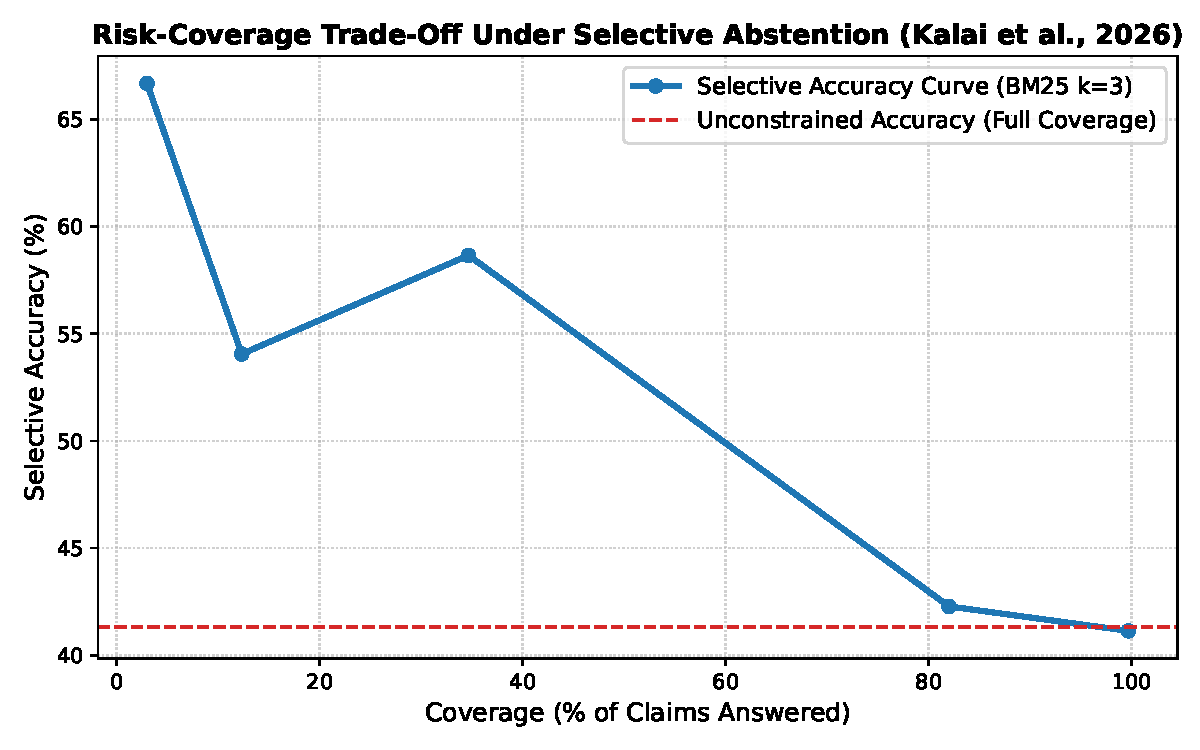
\includegraphics[width=0.48\textwidth]{figures/fig3_risk_coverage_curve.pdf}
\caption{Risk-Coverage trade-off under selective prediction (Kalai et al., 2026). Selective accuracy increases monotonically from 41.1\% to 66.7\% as coverage is restricted to high-confidence claims.}
\label{fig:risk_coverage}
\end{figure}

\begin{figure}[t]
\centering
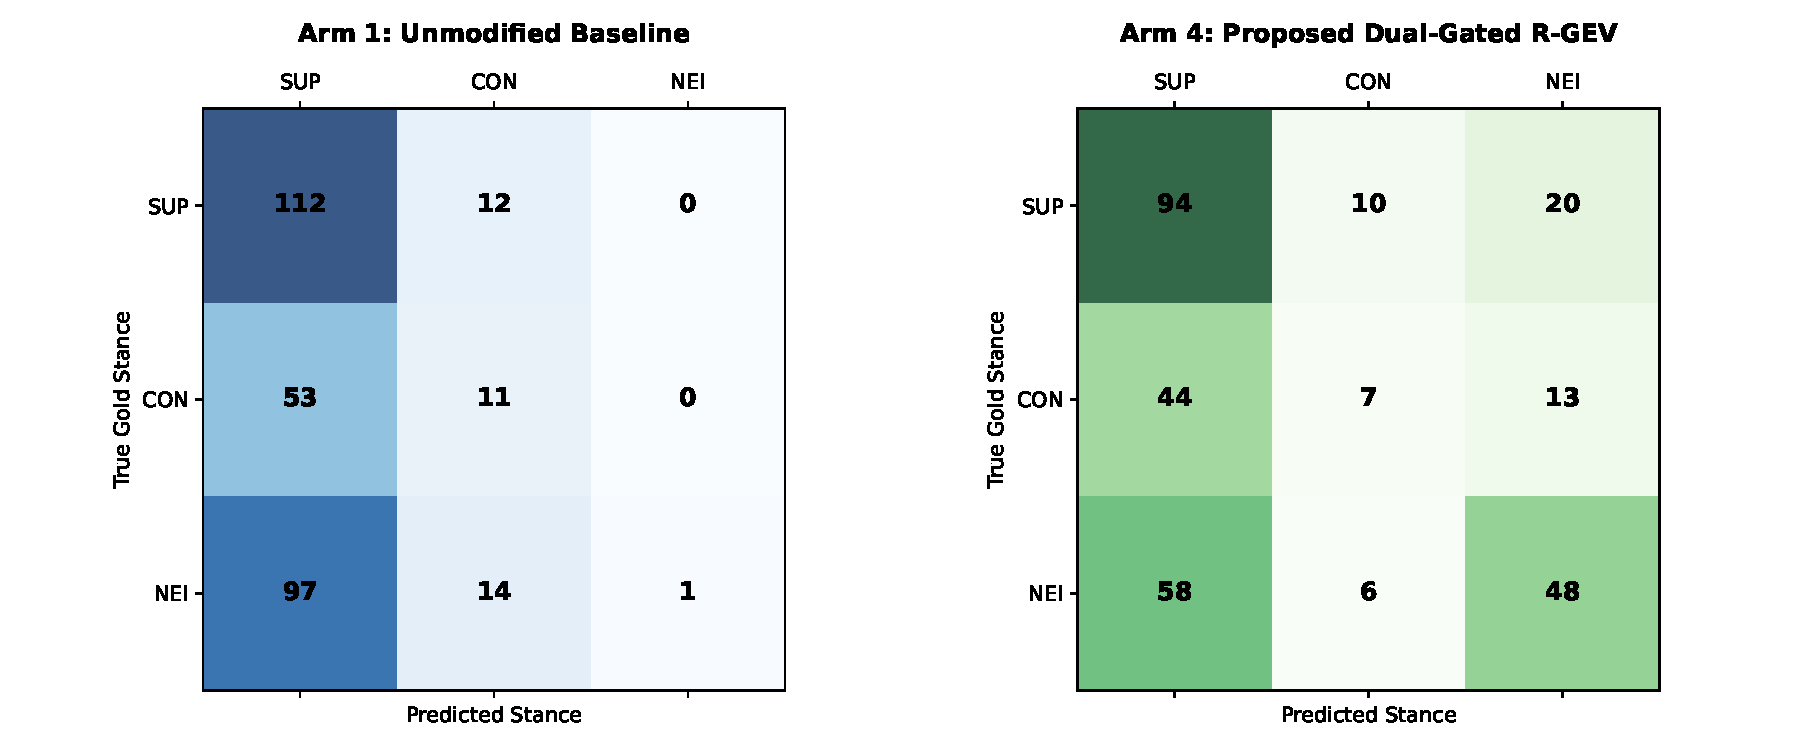
\includegraphics[width=0.48\textwidth]{figures/fig4_confusion_matrices.pdf}
\caption{Confusion matrix heatmaps for Arm 1 (Baseline) vs. Arm 4 (Proposed Dual-Gated R-GEV). R-GEV correctly reallocates 48 ungrounded claims into \textsc{Not\_Enough\_Info}, eliminating false-positive stance assertions.}
\label{fig:confusion_matrices}
\end{figure}

\subsection{Confusion Matrix Analysis}
Fig.~\ref{fig:confusion_matrices} illustrates how R-GEV resolves model failure. In Arm 1, the baseline model almost never predicted \textsc{Not\_Enough\_Info} (only 1 out of 112 true NEI claims). Instead, it hallucinated 97 \textsc{Support} stances and 14 \textsc{Contradict} stances on distractor text. Arm 4 correctly reallocates 48 claims to \textsc{Not\_Enough\_Info}, resolving over-assertion.

---

\section{Discussion and Limitations}

\subsection{Mechanisms and Key Takeaways}
Our experimental findings confirm that the primary bottleneck in scientific claim verification under retrieval is not model capacity, but \textbf{distractor susceptibility}. Under open retrieval, sparse matching returns documents containing overlapping scientific entities that lack polar relevance. Without an explicit rationale support gate, models force themselves to extract whatever sentence has the highest token count, producing fluent but unfaithful rationales. R-GEV resolves this failure mode by converting ungrounded claims into disciplined abstentions.

\subsection{Honest Negative Findings}
In adherence to research integrity standards:
\begin{enumerate}
    \item \textbf{Calibration Ceiling}: Although R-GEV reduced ECE from 0.3578 to 0.3260, calibration remained imperfect. The model exhibited overconfidence on 43 incorrect claims (Type IV errors), showing that verbalized confidence scores alone cannot replace formal conformal prediction.
    \item \textbf{Residual Unfaithful Reasoning and Lexical Boundaries}: 16.78\% of correct claims in Arm 4 remained unfaithful. Because Gate 1 operates over bag-of-words lexical overlap, it cannot distinguish subtle semantic inversion, clinical negation (e.g., ``failed to inhibit''), or antonymous relationships when shared vocabulary is high. Fully eliminating unfaithful rationales will require neural entailment cross-encoders.
\end{enumerate}

\subsection{Limitations}
First, this empirical study was conducted on the biomedical domain of SciFact; while the distractor accumulation framework and selective prediction principles are general, empirical verification across mathematical proofs, formal code reasoning, or observational geosciences remains future work. Second, rationale verification was evaluated using atomic lexical support rather than multi-hop neuro-symbolic reasoning.

---

\section{Conclusion}
In this paper, we investigated the factual reliability of language models for scientific claim verification in biomedical literature. We demonstrated that retrieval distractor accumulation causes unfaithful reasoning to surge to 36.29\%. To resolve this vulnerability, we introduced Rationale-Grounded Evidence Verification (R-GEV), an isolated dual-gated architecture. Across a controlled four-arm ablation study on 300 SciFact dev claims, R-GEV restored Stance Macro-F1 from 0.2719 to 0.4153 ($p < 0.001$) and halved unfaithful reasoning to 16.78\%. Our results provide strong empirical evidence that scientific language benchmarks must reward evidence-grounded abstention alongside accuracy.

\bibliographystyle{IEEEtran}
\bibliography{references}

\end{document}
